\section{Running NEXMD}

NEXMD is a command-line program which always uses a main input file named \verb+input.ceon+, and rarely requires additional input files. The typical workflow is constructing the input in a fresh directory and calling the program as:

\vspace{0.5cm}
\verb+/path_to_nexmd_bin/nexmd.exe > md.out &+
\vspace{0.5cm}

and it is possible to use a main input file with a non-standard name with

\vspace{0.5cm}
\verb+/path_to_nexmd_bin/nexmd.exe < custom_input.ceon > md.out &+
\vspace{0.5cm}
.

Several output files (in addition to the standard output which above is written to \verb+md.out+) will be generated depending on the input parameters. More details about the output files content and format can be found in section 6 of this manual.

Example NEXMD \verb+input.ceon+ files with the expected output are present in the test directory found at
\verb+<NEXMD directory>/tests+. These examples cover most of the features present in NEXMD. It is advised to use these examples to test the NEXMD immediately after compilation. Furthermore, when building a new \verb+input.ceon+ file, it is also advised to use as template one of the \verb+input.ceon+ in the \verb+tests+ directory or in this manual, and modify only the necessary parameters for activating the desired features. This minimal changes are intended to avoid combinations of input keywords that are not benchmarked, not physically justified, or are partially ignored by the sequential reading of keywords as a safeguard to reduce wasting computational resources.

It is also important to notice that there are three mutually-exclusive calculations that NEXMD can perform, enforced by the sequential reading of the main input file. These are optimization, normal modes calculation and molecular dynamics propagation. A main input file suggesting to perform more than one of these calculations will result in an error written to standard output.

Among NEXMD output files, there is one named \verb+restart.out+ written for all the molecular dynamics flavors, which is an input file for restarting the dynamics. If such file is present, NEXMD will restart the simulation from the last molecular dynamics step. The program can be called in a similar way:

\vspace{0.5cm}
\verb+/path_to_nexmd_bin/nexmd.exe < input.ceon >> md.out &+
\vspace{0.5cm}

or

\vspace{0.5cm}
\verb+/path_to_nexmd_bin/nexmd.exe < restart.out >> md.out &+
\vspace{0.5cm}

Note the \verb+>>+ before \verb+md.out+ to append instead of overwriting the standard output file. More details about restarting can be found in section 7 of this manual.

The usual NEXMD workflow when doing research can be followed in Figure \ref{general_flow}. Each of these steps is either an individual run, a set of individual runs, or the analysis of a set of output files.

\begin{figure}[ht]
	\centering
	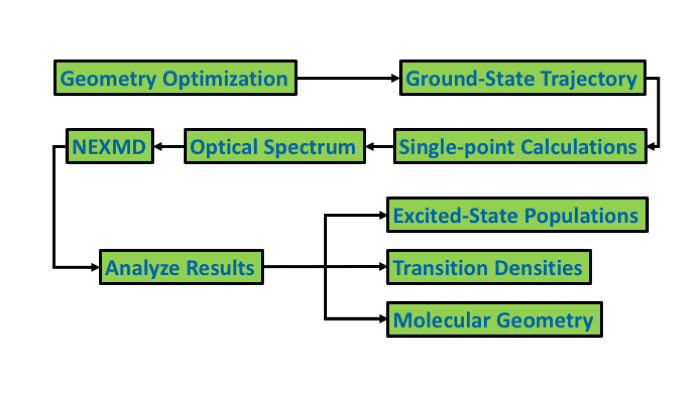
\includegraphics[scale=.6]{general_procedure.png}
	\caption{\small A schematic of the general procedure for simulating non-adiabatic dynamics.}\label{general_flow}
\label{genproc}
\end{figure}